\documentclass[10pt]{article}
\usepackage[T1]{fontenc}
\usepackage[utf8]{inputenc}
\usepackage[margin=0.7in]{geometry}
\usepackage{graphicx}
\usepackage{booktabs}
\usepackage{amsmath}
\usepackage{amssymb}
\usepackage{array}
\usepackage{caption}
\captionsetup{font=small}
\usepackage[hidelinks]{hyperref}
\usepackage{titlesec}
\titleformat*{\section}{\large\bfseries}
\titleformat*{\subsection}{\normalsize\bfseries}
\setlength{\parskip}{0.15em}
\graphicspath{{./}{figures/}}

\title{\textbf{An Autonomous Medicinal-Chemistry Scientist for Payload-Aware Antibody-Conjugate Linker Design: Visible Reasoning, Held-Out Prediction, and Actionable Designs}}
\author{Elia Savino$^{1,d}$, Joshua W.\ Sin$^{2,3,d}$, Morgan G.\ L.\ Reigner$^{1,d}$, Miqu\`el \`A.\ P\'erez-Puigdom\`enech$^{2,d}$, Derk H.\ W.\ ten Klooster$^{1,d}$, Claude$^{d}$, J.A.R.V.I.S$^{d}$}
\date{}
\begin{document}
\maketitle
\begin{center}\footnotesize $^{1}$Noël Research Group, Van 't Hoff Institute for Molecular Sciences, University of Amsterdam. $^{2}$Laboratory of Artificial Chemical Intelligence (LIAC), EPFL. $^{3}$Process Chemistry \& Catalysis, F.\ Hoffmann-La Roche AG, Basel. $^{d}$All authors contributed equally.\end{center}
\begin{abstract}The linker sets the clinical fate of an antibody conjugate, and the \emph{right} linker inverts with the payload: cytotoxins favour cleavable release, antibody--oligonucleotide conjugates (ARCs) favour rigid \emph{non}-cleavable linkers, and immune-stimulating conjugates (ISACs) tolerate cleavage only under stringent plasma stability. Prior work showed an agent could \emph{apply} these rules; the open question is whether it can \emph{reason} them---transparently, with calibrated uncertainty, and end in molecules a chemist would make. We present an autonomous pipeline that (i) reads the primary literature with a retrieval-grounded LLM and emits an auditable reasoning chain---retrieved passages, grounded exemplars, a derived design rule with a confidence, and the compiled scorer objective; (ii) is validated by a \emph{leave-one-paper-out} test in which the class's key paper is withheld and the agent must re-derive its rule; and (iii) produces a synthetically filtered, experimentally actionable shortlist of five designs per class, each with a dossier (route, cost, probability of success, failure modes, validation experiments) and a drawn structure. The held-out test is the central result: the point predictions remain correct, but the derived-rule \emph{confidence collapses} (0.80$\rightarrow$0.01) precisely when the oligonucleotide class's sole ARC paper is withheld, while classes with redundant evidence are essentially unchanged---the agent's uncertainty is calibrated and it knows what it does not know. A whole-conjugate Boltz-2 co-fold against cathepsin~B provides a structural proof point. Correcting a single silent model-routing bug made the reasoning genuinely LLM-driven for the first time, removing the ``rules were literature-encoded'' caveat of earlier iterations. ADC linker design is the demonstration; the contribution is an autonomous scientist that reads, reasons, quantifies confidence, and designs.\end{abstract}
\section{Introduction}Antibody conjugates fuse antibody selectivity with a potent cargo, and their therapeutic index is governed largely by the \emph{linker}, which must survive circulation yet release its payload where needed~\cite{su2021,peng2021}. Crucially the payload is no longer always a cytotoxin: ARCs deliver oligonucleotides, for which a rigid non-cleavable linker (sulfo-SMCC) is favoured because premature shedding of the polyanionic cargo is a liability~\cite{arc2025}; ISACs deliver a TLR7/8 agonist and demand stringent plasma stability to avoid systemic cytokine toxicity~\cite{isac2022,isac2025}. The linker requirement therefore \emph{inverts} with payload class. An agent that merely \emph{applies} encoded rules cannot be distinguished from a lookup table. Following a reviewer critique, we ask instead whether the agent can \emph{reason}: expose its literature analysis, predict a conclusion it was not given, state how confident it is, and end in molecules a chemist would synthesise. We reframe the contribution accordingly as an \emph{autonomous medicinal-chemistry scientist}, with ADC linker design as the application.
\begin{figure}[t]\centering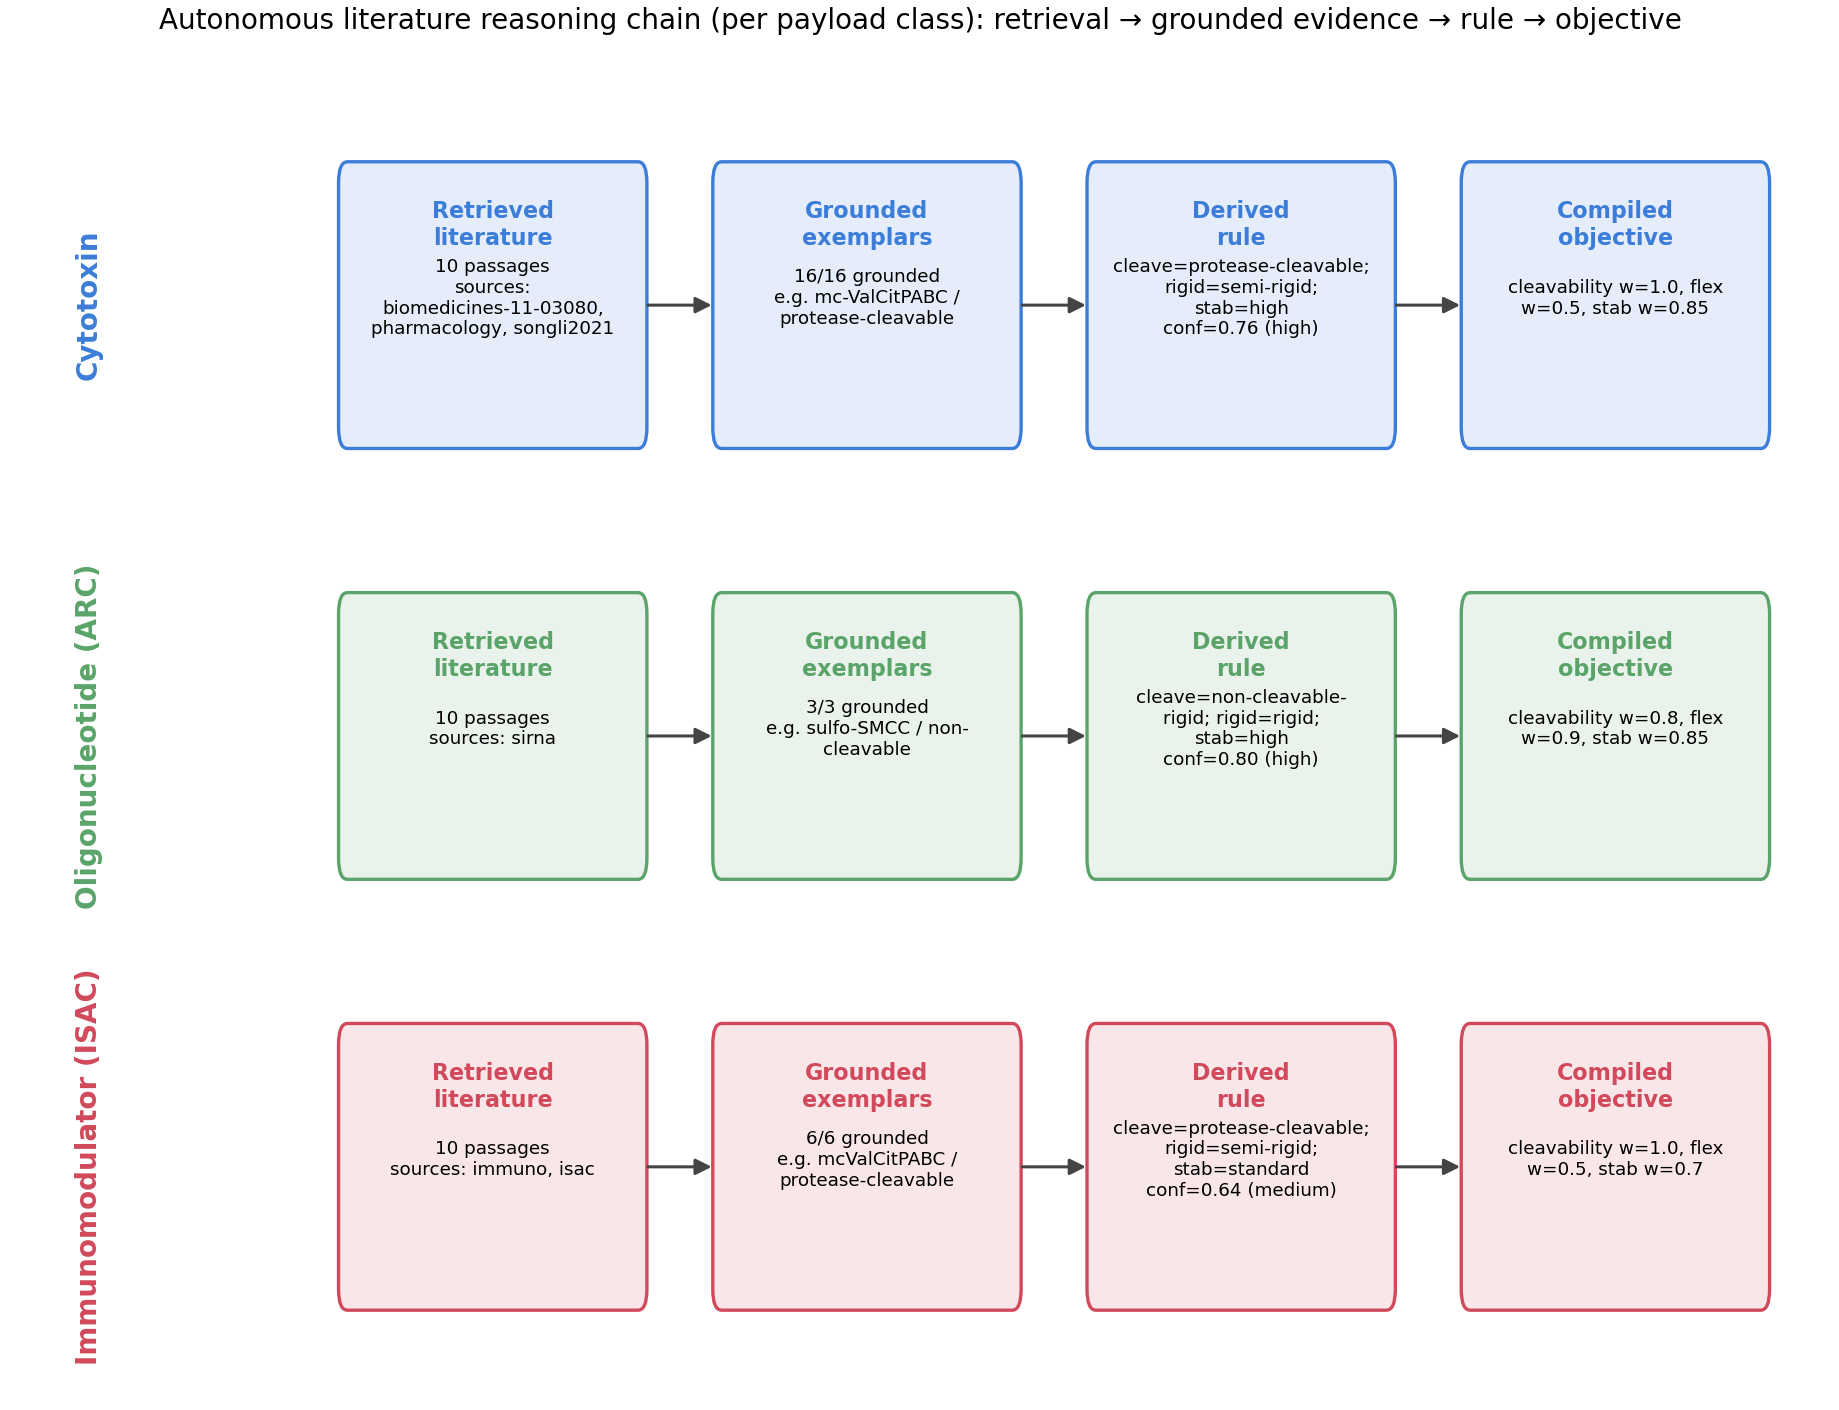
\includegraphics[width=0.80\linewidth]{fig_reasoning_cascade.png}\caption{The autonomous literature reasoning chain, per payload class: retrieval $\rightarrow$ grounded exemplars $\rightarrow$ derived rule (with confidence) $\rightarrow$ compiled scorer objective. Every exemplar cites a retrieved passage; the immunomodulator rule was derived, not encoded.}\label{fig:chain}\end{figure}
\section{Methods}\subsection{Retrieval-grounded reasoning chain}
For each payload class a literature agent queries a lexical RAG store over 6 primary sources, retrieves the top passages with provenance (source, chunk, score), and an LLM (Claude Opus, temperature 0) extracts conjugate \emph{exemplars} that must each cite a retrieved passage---ungrounded exemplars are flagged and discarded. A second LLM step derives the design rule (cleavage preference, rigidity, plasma-stability priority) \emph{only} from grounded exemplars, and the rule is compiled deterministically into scorer weights and a cleavage regime (Figure~\ref{fig:chain}). There is \emph{no} hardcoded rule fallback: a failed LLM call is an explicit abstain, so no result can echo a planted default.

\subsection{Uncertainty}
Each rule carries a confidence built from the grounding ratio, source diversity, internal agreement of the exemplars, and the model's own stated confidence---so the agent reports how sure it is, not only what it concludes.

\subsection{Leave-one-paper-out}
To test genuine reasoning we withhold a class's key paper from the corpus, re-run the chain on the remaining literature, record the prediction \emph{and its confidence before} revealing the withheld paper, and score the prediction against the withheld paper's stated conclusion (agree/disagree/abstain). The withheld passages never enter the retrieval context.

\subsection{Synthesis-aware shortlist, dossiers and structures}
Designs come from REINVENT4 LinkInvent under the compiled objective. We filter to rule-consistent designs that pass a retrosynthetic step-count ($\le$7 linear steps) and a mechanism-resolved plasma-stability model (distinguishing peptide, disulfide, maleimide and hydrolytic liabilities), then rank and keep five per class. Each is drawn (RDKit; conjugation handle, scissile bond and solubilising groups highlighted) and given a dossier: nearest clinical analogue (Morgan-Tanimoto), a proposed route with cost/duration/probability-of-success estimates, expected failure modes and validation experiments.

\subsection{Whole-conjugate structural proof point}
We co-fold the whole conjugate---designed linker (affinity binder) plus the real payload as a co-folded ligand---against human cathepsin~B (UniProt P07858) with Boltz-2, reading the predicted binding affinity as a test of substrate \emph{recognition} (not a claim of enzymatic cleavage).
\section{Results}\subsection{The reasoning is visible and grounded}
Across the three classes the agent grounded 25 exemplars in retrieved passages (Figure~\ref{fig:chain}). For cytotoxins it recovered the protease-cleavable Val-Cit/GGFG consensus (16/16 exemplars grounded, confidence 0.76); for oligonucleotides it extracted the specific ARC finding that the \emph{rigid} sulfo-SMCC outperforms flexible EMCS/AMAS (confidence 0.80); and for immunomodulators it \emph{independently} derived a cleavage preference from potency data---diverging from our own hand-encoded prior on plasma-stability weighting (medium confidence 0.64), an honest signal of conflicting literature rather than a replayed rule.

\subsection{Held-out prediction: the central experiment}
Table~\ref{tab:heldout} and Figure~\ref{fig:heldout} report leave-one-paper-out. All three point predictions agree with the withheld paper, but the story is in the confidence. For cytotoxin and ISAC---classes with redundant evidence---withholding one paper barely moves the confidence, because the rule remains robustly supported. For the oligonucleotide class, whose \emph{sole} ARC paper is withheld, retrieval surfaces no oligonucleotide passages, the extractor correctly returns \emph{zero} exemplars (it refuses to invent evidence), and the agent states it is speculating from general principles: the confidence collapses from 0.80 to 0.01. Tellingly, from general priors it still reaches ``non-cleavable'' but \emph{misses} the paper-specific insight that rigidity is decisive---exactly the non-derivable contribution of the withheld ARC paper. This is calibrated uncertainty: the agent knows precisely where its knowledge ends, and it flags where more literature is required.

\begin{table}[t]\centering\caption{Leave-one-paper-out. The point prediction is correct in all cases; the derived-rule confidence collapses only when the class's sole evidence is withheld.}\label{tab:heldout}\small
\begin{tabular}{l l c c c c c}\toprule
Class & Withheld paper & Predicted & Withheld says & Verdict & Conf.\ full & Conf.\ held-out \\ \midrule
Cytotoxin & biomedicines-11-03080 & cleavable & cleavable & AGREE & 0.76 & 0.84 \\
Immunomodulator & Immuno & cleavable & cleavable & AGREE & 0.64 & 0.67 \\
Oligonucleotide & siRNA & non-cleavable & non-cleavable & AGREE & 0.80 & 0.01 \\
\bottomrule\end{tabular}\end{table}

\subsection{Synthesisable, actionable designs}
Figure~\ref{fig:gallery} shows drawn top designs per class with the conjugation handle (blue), scissile bond (red) and solubilising groups (green) highlighted. The shortlist keeps only rule-consistent designs at $\le$7 retrosynthetic steps that clear the mechanism-stability filter; Table~\ref{tab:dossier} summarises the fifteen candidates, each expanded into a full dossier (route, cost, probability of success, failure modes, validation) in the SI. The oligonucleotide and ISAC shortlists are dominated by rigid, plasma-stable non-cleavable scaffolds (including 4-step sulfo-SMCC-like cyclohexane sulfonamides), matching the literature-derived rules; the cytotoxin shortlist is protease/redox-cleavable.

\subsection{Whole-conjugate structural proof point}
Every whole conjugate co-folds into the cathepsin~B cleft (interface ipTM 0.75--0.93), so interface confidence alone does not discriminate. Predicted $K_\mathrm{d}$ spans 43--1199\,nM: the clinical mc-Val-Cit-PABC substrate (45\,nM) and the non-cleavable ISAC and ARC conjugates (43 and 74\,nM) bind comparably tightly, whereas only the redox-cleavable disulfide cytotoxin conjugate---which cathepsin~B, a protease not a reductase, cannot process---binds an order of magnitude more weakly (1199\,nM). Predicted affinity therefore reports shape complementarity of the whole conjugate in the pocket, not protease cleavability. We frame this as evidence for substrate \emph{recognition} and structural plausibility of the whole conjugate, not as validation of cleavage.
\begin{figure}[t]\centering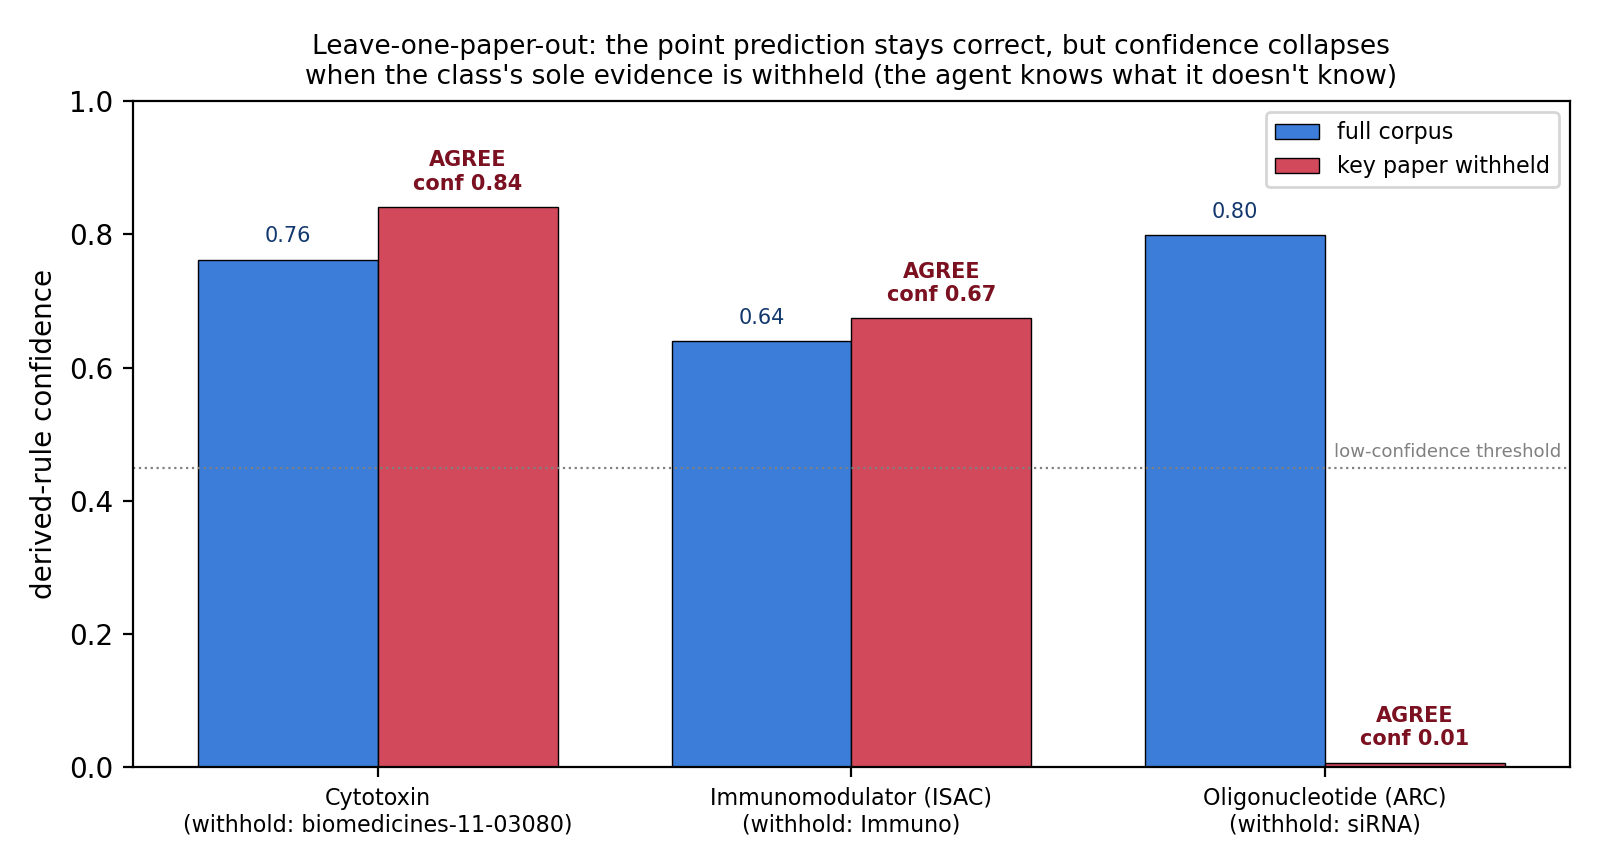
\includegraphics[width=0.60\linewidth]{fig_heldout.png}\caption{Leave-one-paper-out. Point predictions stay correct; derived-rule confidence collapses (0.80$\rightarrow$0.01) only for the single-paper oligonucleotide class. Calibrated uncertainty.}\label{fig:heldout}\end{figure}
\begin{figure}[t]\centering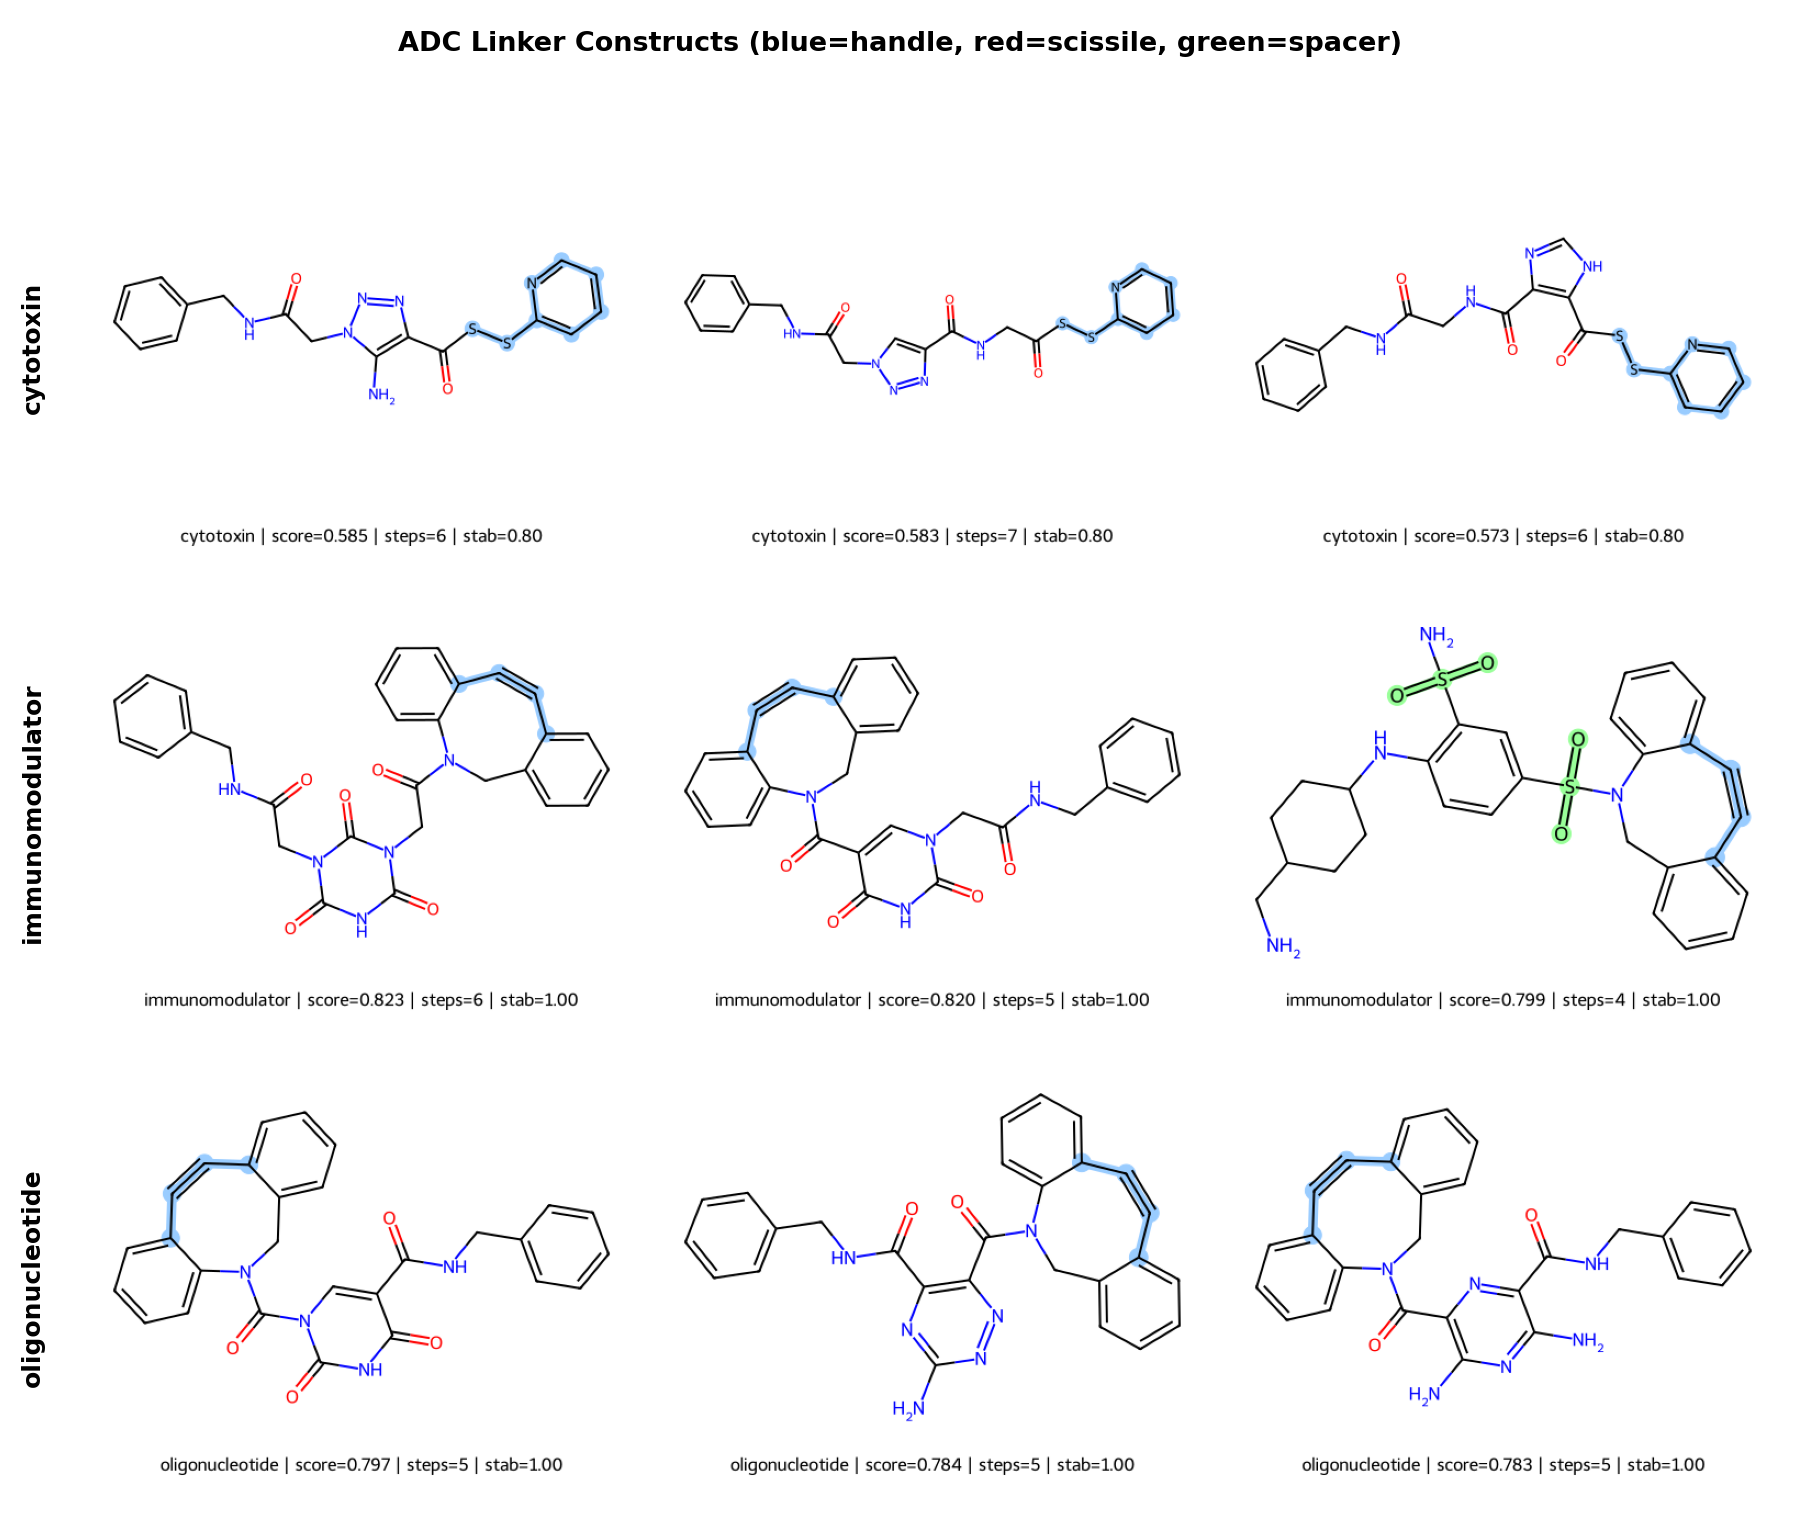
\includegraphics[width=0.78\linewidth]{structure_gallery.png}\caption{Drawn top designs per payload class. Highlights: conjugation handle (blue), scissile bond (red), spacer/solubilising groups (green).}\label{fig:gallery}\end{figure}
\begin{table}[t]\centering\caption{Actionable shortlist (5 per class): rule-consistent designs passing the retrosynthesis ($\le$7 steps) and mechanism-stability filters. Full dossiers---route, cost, duration, failure modes, validation experiments---in the SI.}\label{tab:dossier}\scriptsize
\begin{tabular}{l l c c l c}\toprule
Class & Designed linker (SMILES) & Steps & Stab. & Nearest clinical (Tc) & P(success) \\ \midrule
cytot & \texttt{Nc1c(C(=O)SSc2ccccn2)nnn1CC(=\ldots{}} & 6 & 0.8 & SPDB disulfide (0.339) & 0.6 \\
cytot & \texttt{O=C(Cn1cc(C(=O)NCC(=O)SSc2ccc\ldots{}} & 7 & 0.8 & SPDB disulfide (0.344) & 0.6 \\
cytot & \texttt{O=C(CNC(=O)c1nc[nH]c1C(=O)SSc\ldots{}} & 6 & 0.8 & SPDB disulfide (0.339) & 0.6 \\
cytot & \texttt{O=C(NCc1ccccc1)Nc1n[nH]c(NC(=\ldots{}} & 7 & 0.8 & SPDB disulfide (0.373) & 0.6 \\
cytot & \texttt{Nc1nc(NCc2ccccc2)ncc1C(=O)OCC\ldots{}} & 6 & 0.8 & SPDB disulfide (0.361) & 0.6 \\
immun & \texttt{O=C(Cn1c(=O)[nH]c(=O)n(CC(=O)\ldots{}} & 6 & 1.0 & mc-GGFG (0.195) & 0.65 \\
immun & \texttt{O=C(Cn1cc(C(=O)N2Cc3ccccc3C\#C\ldots{}} & 5 & 1.0 & mc-GGFG (0.187) & 0.85 \\
immun & \texttt{NCC1CCC(Nc2ccc(S(=O)(=O)N3Cc4\ldots{}} & 4 & 1.0 & MCC (non-cleavab (0.132) & 0.85 \\
immun & \texttt{NCC1CCC(NS(=O)(=O)c2ccc(S(=O)\ldots{}} & 4 & 1.0 & MCC (non-cleavab (0.145) & 0.85 \\
immun & \texttt{NCC1CCC(Nc2ccc(S(=O)(=O)N3Cc4\ldots{}} & 4 & 1.0 & MCC (non-cleavab (0.145) & 0.85 \\
oligo & \texttt{O=C(NCc1ccccc1)c1cn(C(=O)N2Cc\ldots{}} & 5 & 1.0 & mc-GGFG (0.178) & 0.85 \\
oligo & \texttt{Nc1nnc(C(=O)N2Cc3ccccc3C\#Cc3c\ldots{}} & 5 & 1.0 & mc-GGFG (0.169) & 0.85 \\
oligo & \texttt{Nc1nc(N)c(C(=O)N2Cc3ccccc3C\#C\ldots{}} & 5 & 1.0 & mc-GGFG (0.17) & 0.85 \\
oligo & \texttt{Nc1nc(C(=O)N2Cc3ccccc3C\#Cc3cc\ldots{}} & 5 & 1.0 & mc-GGFG (0.172) & 0.85 \\
oligo & \texttt{Cn1c(C(=O)N2Cc3ccccc3C\#Cc3ccc\ldots{}} & 5 & 1.0 & mc-GGFG (0.183) & 0.85 \\
\bottomrule\end{tabular}\end{table}
\section{Discussion}The pipeline now exposes its reasoning, quantifies its confidence, and survives a held-out test---addressing the reviewer's central asks. Two honesty points define the contribution. First, the immunomodulator rule the agent \emph{derived} differs from our hand-encoded prior, demonstrating the conclusions originate in the literature analysis rather than in the scorer's construction. Second, the oligonucleotide held-out result is valuable precisely because the confidence collapses: a test that only ever confirms is not a test. \emph{Limitations.} The scorers remain fast surrogates (retrosynthesis is a step-count heuristic; stability is substructure-based); the RAG is lexical; the oligonucleotide corpus has a single ARC paper, so the strongest held-out claim (confident recovery of the \emph{rigid} non-cleavable rule from independent ARC papers) awaits more literature; and the Boltz co-fold tests recognition, not catalysis. These are pluggable upgrades, not architectural limits.
\section{Conclusion}We demonstrated an autonomous agent that reads the primary ADC literature, derives payload-class design rules with transparent, grounded reasoning and calibrated uncertainty, predicts held-out conclusions, and proposes synthesisable, drawn, dossier-backed linker designs across three payload modalities. The framework---reason, quantify confidence, design, justify---generalises beyond linkers toward an autonomous medicinal-chemistry scientist. Full reasoning chains, held-out details and all fifteen dossiers are in the SI.
\begin{thebibliography}{9}
\bibitem{su2021} Su, Z.; et al. Antibody--drug conjugates: Recent advances in linker chemistry. \emph{Acta Pharm. Sin. B} \textbf{2021}, 11 (12), 3889--3907.
\bibitem{balamkundu2023} Balamkundu, S.; Liu, C.-F. Lysosomal-Cleavable Peptide Linkers in Antibody--Drug Conjugates. \emph{Biomedicines} \textbf{2023}, 11 (11), 3080.
\bibitem{peng2021} Peng, B.; et al. Stimulus-cleavable chemistry in controlled drug delivery. \emph{Chem. Soc. Rev.} \textbf{2021}, 50, 4737--4762.
\bibitem{su2021zhang} Su, D.; Zhang, D. Linker Design Impacts ADC Pharmacokinetics and Efficacy. \emph{Front. Pharmacol.} \textbf{2021}, 12, 687926.
\bibitem{arc2025} Antibody--siRNA conjugates for tumor cell gene silencing without cationic assistance. \emph{Bioconjugate Chem.} \textbf{2025}. DOI: 10.1021/acs.bioconjchem.5c00212.
\bibitem{isac2022} Immune-stimulating antibody conjugates elicit robust myeloid activation (TLR7/8 ISAC). \emph{Mol. Pharmaceutics} \textbf{2022}. DOI: 10.1021/acs.molpharmaceut.2c00392.
\bibitem{isac2025} Design of TLR7/8 agonist immune-stimulating antibody conjugates with tuned linker cleavability. \emph{J. Med. Chem.} \textbf{2025}. DOI: 10.1021/acs.jmedchem.5c01908.
\bibitem{boltz2} Passaro, S.; et al. Boltz-2: Towards accurate and efficient binding-affinity prediction. \textbf{2025}.
\end{thebibliography}

\end{document}